\documentclass{beamer}
\usetheme{Copenhagen}
\usepackage[utf8]{inputenc}
\usepackage[brazil]{babel}  % Pacote
\usepackage{mflogo}
\usepackage{caption}
\usepackage{minted}
\author{Amadeus Folego}
\title{\LaTeX\ em aplicações Rails}
\date{}
\institute{
  \begin{tabular}{c c}        
    {\em www} & \url{http://badosu.com}\\
    {\em email} & \url{amadeusfolego@gmail.com}
  \end{tabular}
}
\begin{document}
  \begin{frame}[plain] 
    \titlepage
  \end{frame}
  \begin{frame}{Apresentação}
  \end{frame}
  \begin{frame}{Don Knuth}
    \begin{columns}[c]
      \column{.2\textwidth}
        \begin{figure}[t]
          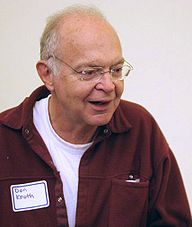
\includegraphics[width=\columnwidth]{192px-KnuthAtOpenContentAlliance}
          \caption*{\scriptsize Donald Ervin Knuth}
        \end{figure}
      \column{.8\textwidth}
        \begin{itemize}
          \item Análise de algoritmos \pause
          \item Números Surreais /w John Conway \pause
          \item Livros \pause
            \begin{itemize}
              \item {\em The Art of Computer Programming (TAOCP) - 1969} \pause
              \item {\em Concrete Mathematics - 1970} \pause 
            \end{itemize}
          \item \MF\pause
          \item \TeX\ 
        \end{itemize}
    \end{columns}
  \end{frame}
  \begin{frame}{\LaTeX\ ?}
    Por quê \LaTeX?\\\pause
    \begin{itemize}
      \item{\fontfamily{cmr}\selectfont Porque é necessária excelência tipográfica!\pause
        \begin{itemize}
          \item Ao receber a prévia da segunda edição do {\em Concrete Mathematics}\pause
        \end{itemize}}
      \item \TeX\ $\implies$ \LaTeX\ \ \ {\scriptsize 1976 Knuth - 1980's Leslie Lamport}\pause
      \item Um dos primeiros projetos de software livre\pause
      \item Comunidade enorme (praticamente a maioria dos cientistas)
    \end{itemize}
  \end{frame}
  \begin{frame}[fragile]{Capacidades}
    \onslide<1,2>{$ \rightarrow $} Conteúdo sobre formatação\pause\ {\scriptsize-- em oposição a \texttt{WYSIWYG}}\\\pause
    \onslide<3>{$ \rightarrow $} Linguagem Turing-Completa\\\pause
    \onslide<4>{$ \rightarrow $} Extremamente extensivo\\\pause
    \onslide<5>{$ \rightarrow $} É apenas texto\\\pause
    \onslide<6->{$ \rightarrow $} Expressões matemáticas\\\pause 
      $$ \oint_{D} B\cdot n\ dS = 0 $$
    \begin{center}
      \onslide<6>\pause\href{doc/rogers}{\beamerbutton{Exemplo}}\\
    \end{center}
\end{frame}
  \begin{frame}[fragile]{Código}
    Comandos da forma: \mint{tex}|  \comando[opcao]{argumento}|\pause
    Fórmulas chamadas por comandos ou cercadas por {\texttt \$}: \mint{tex}|$$ \oint_{D} B\cdot n\ dS = 0 $$|
\end{frame}
  \begin{frame}[fragile]{Código}
    \center {\Large Conteúdo sobre formato}\pause
    \begin{itemize}
    \item Artigo? \pause \mint{tex}|\documentclass{article}|\pause
    \item Livro? \pause \mint{tex}|\documentclass{book}|\pause
    \item Implementar um milhão de regras da abnt? \pause \mint{tex}|\documentclass{abnt}|
            \large{AbnTex {\em (Absurdas Normas em Tex)}}\pause
    \item Fazer o sumário do seu livro quilométrico?\pause \mint{tex}|\tableofcontents|
    \end{itemize}
\end{frame}
  \begin{frame}[fragile]{Código}
    Estrutura básica de um arquivo {\texttt .tex}:
    \begin{minted}{tex}
      \documentclass{beamer}
      \usetheme{Copenhagen}
      \usepackage[utf8]{inputenc}
      \usepackage[brazil]{babel}
      % pacotes, classe de documento, configuracoes macro
    \end{minted}
    \pause\begin{minted}{tex}
      \author{Amadeus Folego}
      \title{\LaTeX\ em aplicacoes Rails}
      % algumas informacoes
    \end{minted}
    \pause\begin{minted}{tex}
      \begin{document}
      % aqui o bicho pega
    \end{minted}
\end{frame}
  \begin{frame}{Desvantagens}
    \onslide<1->{ $ \rightsquigarrow $ } Exige muitas dependências\\\pause
    \onslide<2->{ $ \rightsquigarrow $ } É compilado\\\pause
    \onslide<3> { $ \rightsquigarrow $ } Barreira inicial de aprendizado
  \end{frame}
  \begin{frame}{Motivação} 
    \onslide<1>{$ \nabla $} Mudança de paradigma $\rightarrow$ {\tiny Sites com conteúdo textual $ \implies $ Aplicações Web}\\\pause
    \onslide<2>{$ \nabla $} Geração de Documentos\\\pause
    \onslide<3>{$ \nabla $} Latex é apenas texto\\\pause
    \onslide<4>{$ \nabla $} Quantidade enorme de tipos de documento\\
  \end{frame}
  \begin{frame}{Exemplo prático} 
    \begin{center} 
      {\Huge Exemplo Prático}\\[1em]
      Uma aplicação Web em que o usuário pode criar apresentações, em formato pdf, utilizando a classe de documento beamer.
    \end{center}
  \end{frame}
  \begin{frame}{Mão na massa} 
    \begin{center} 
      \Large Gem {\texttt rails-latex}: \href{https://github.com/jacott/rails-latex}{\beamergotobutton{rails-latex}} 
    \end{center}
  \end{frame}
  \begin{frame}{Requisitos} 
    \begin{center} 
      \begin{itemize}
        \item {\texttt Gemfile}\\\mint{ruby}|gem 'rails-latex'|
        \item {\texttt config/initializers/mime\_types.rb}\\{\scriptsize \mint{ruby}|Mime::Type.register "application/pdf", :pdf, ['text/pdf'], ['pdf']|}
        \item {\texttt app/views/layouts/application.pdf.erbtex}
        \item {\texttt app/views/controller/action.pdf.erb}
      \end{itemize}
    \end{center}
  \end{frame}
  \begin{frame}[plain] 
    \titlepage
  \end{frame}
\end{document}
